\begin{figure*}[t]
\vskip 0.2in
\begin{center}
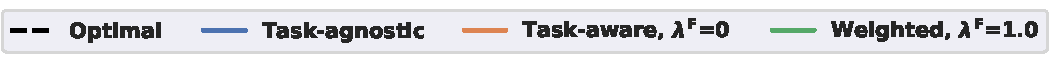
\includegraphics[width=0.8\columnwidth]{figures/main_legend.pdf}
%\subfigure[]{
\subfigure{
{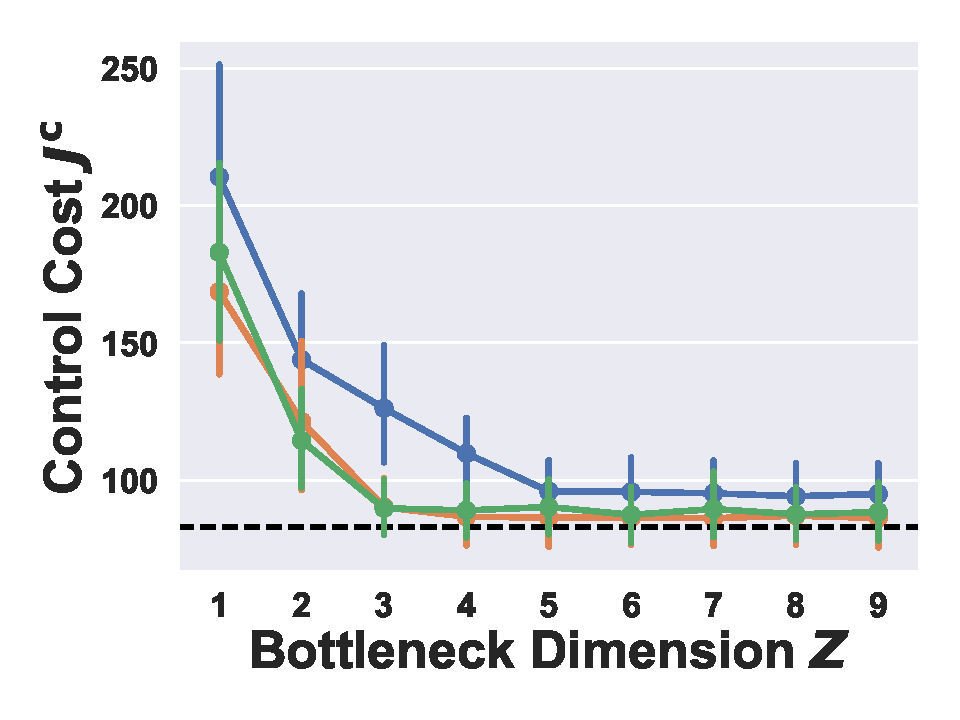
\includegraphics[width=0.31\columnwidth]{figures/iot/iot_cost_bottleneck.pdf}}
\label{fig_iot_cost_bottleneck}
}
%\subfigure[]{
\subfigure{
{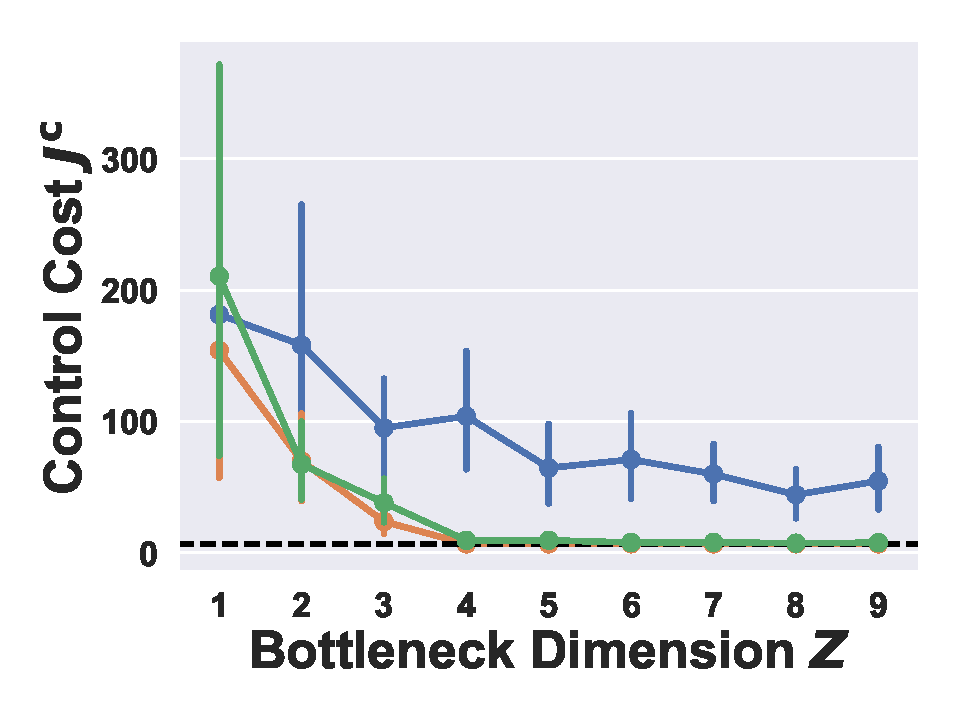
\includegraphics[width=0.31\columnwidth]{figures/cell/cell_cost_bottleneck.pdf}}
\label{fig_cell_cost_bottleneck}
}
%\subfigure[]{
\subfigure{
{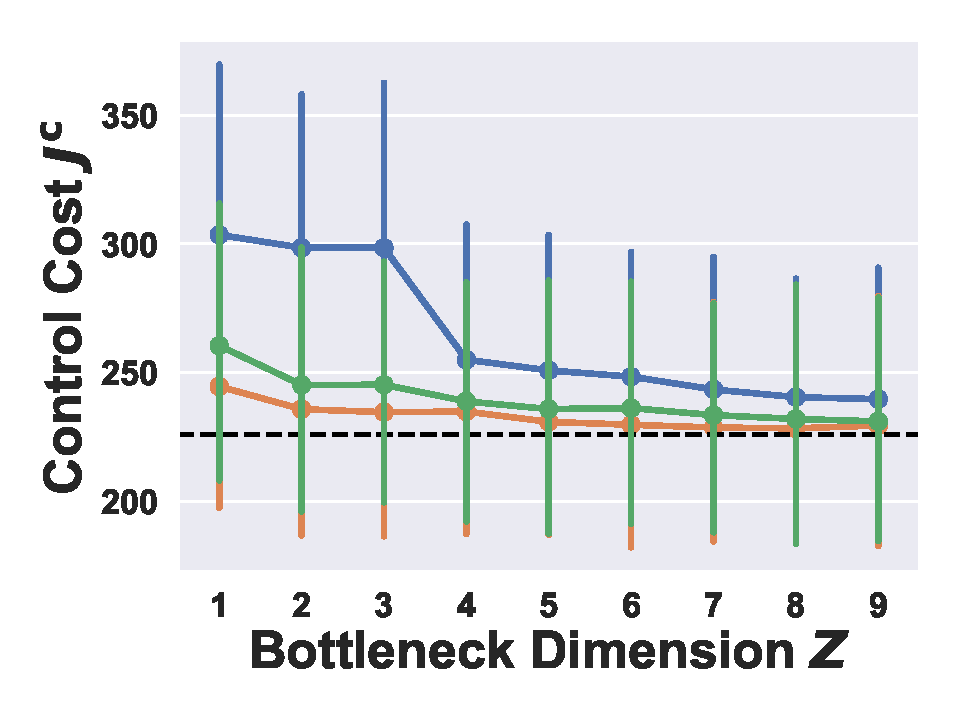
\includegraphics[width=0.31\columnwidth]{figures/pjm/pjm_cost_bottleneck.pdf}}
\label{fig_pjm_cost_bottleneck}
}
%\subfigure[]{
\subfigure{
{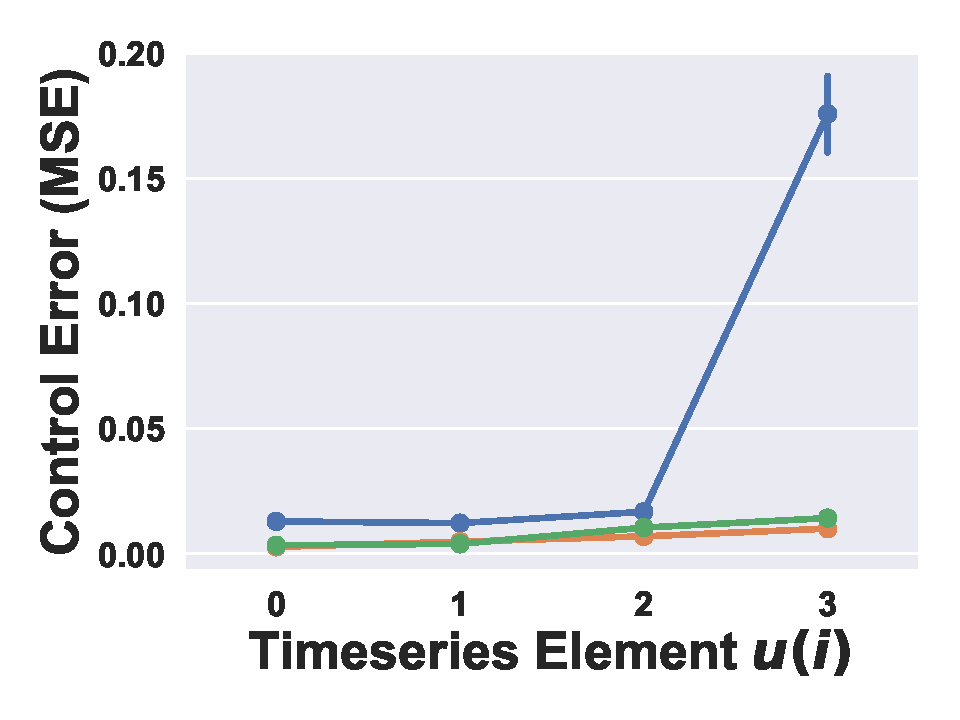
\includegraphics[width=0.31\columnwidth]{figures/iot/control_errors.pdf}}
\label{fig_iot_control_errors}
}
%\subfigure[]{
\subfigure{
{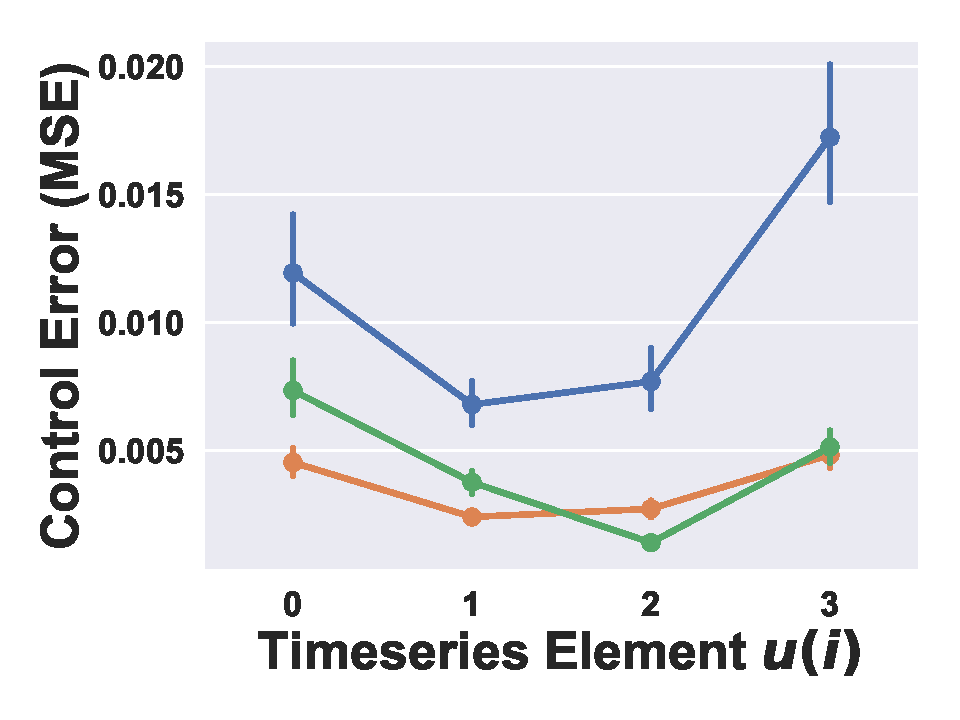
\includegraphics[width=0.31\columnwidth]{figures/cell/control_errors.pdf}}
\label{fig_cell_control_errors}
}
%\subfigure[]{
\subfigure{
{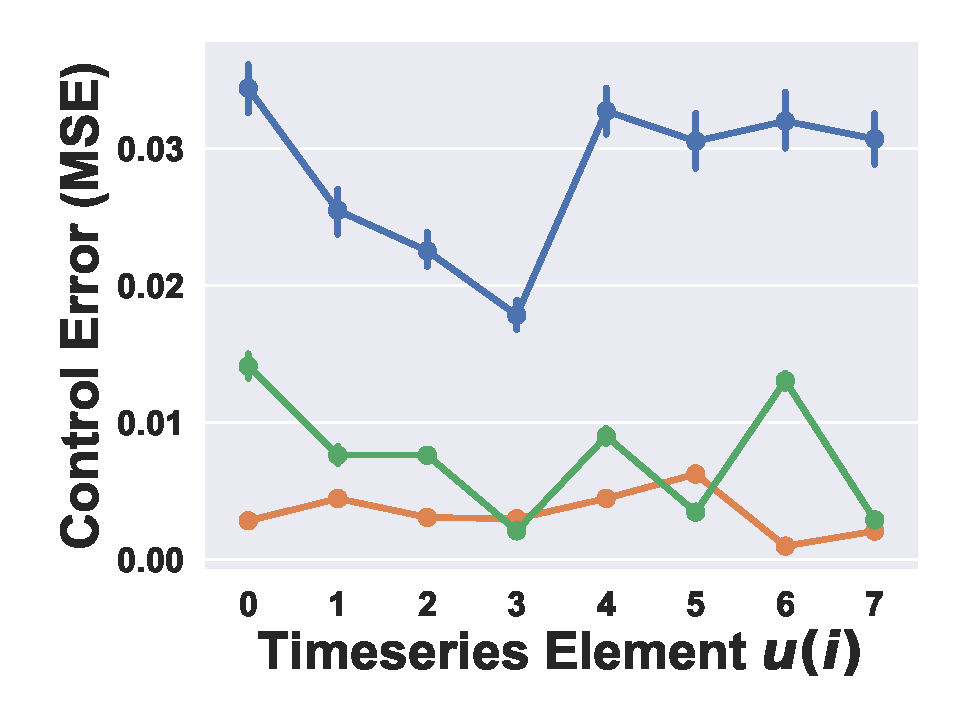
\includegraphics[width=0.31\columnwidth]{figures/pjm/control_errors.pdf}}
\label{fig_pjm_control_errors}
}
%\subfigure[]{
\subfigure{
{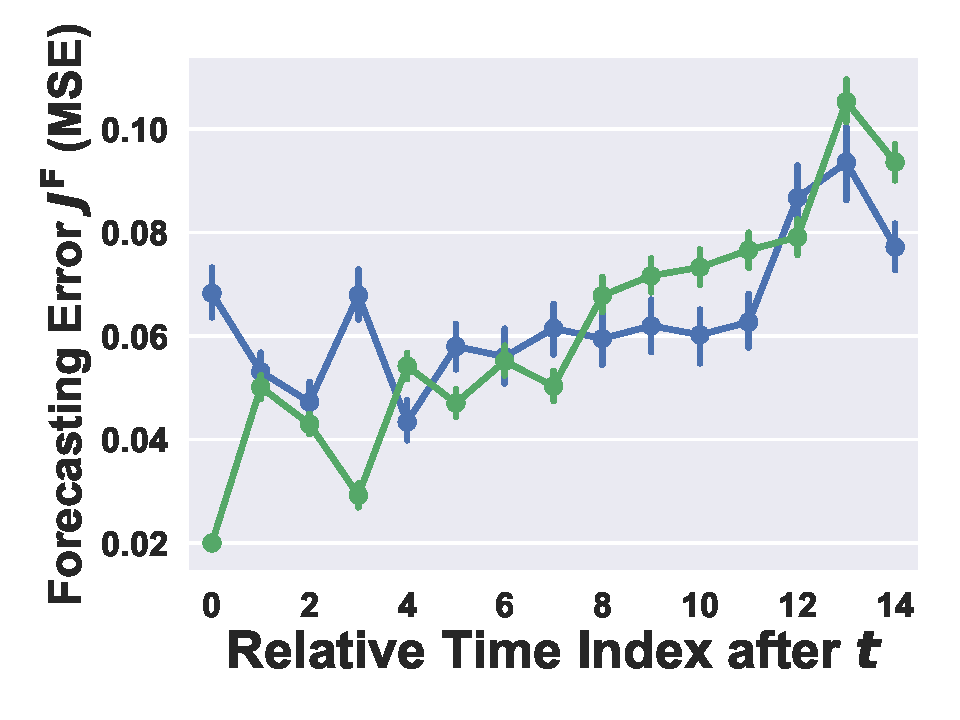
\includegraphics[width=0.31\columnwidth]{figures/iot/forecast_errors_time_horizon.pdf}}
\label{fig_iot_forecast_errors_time_horizon}
}
%\subfigure[]{
\subfigure{
{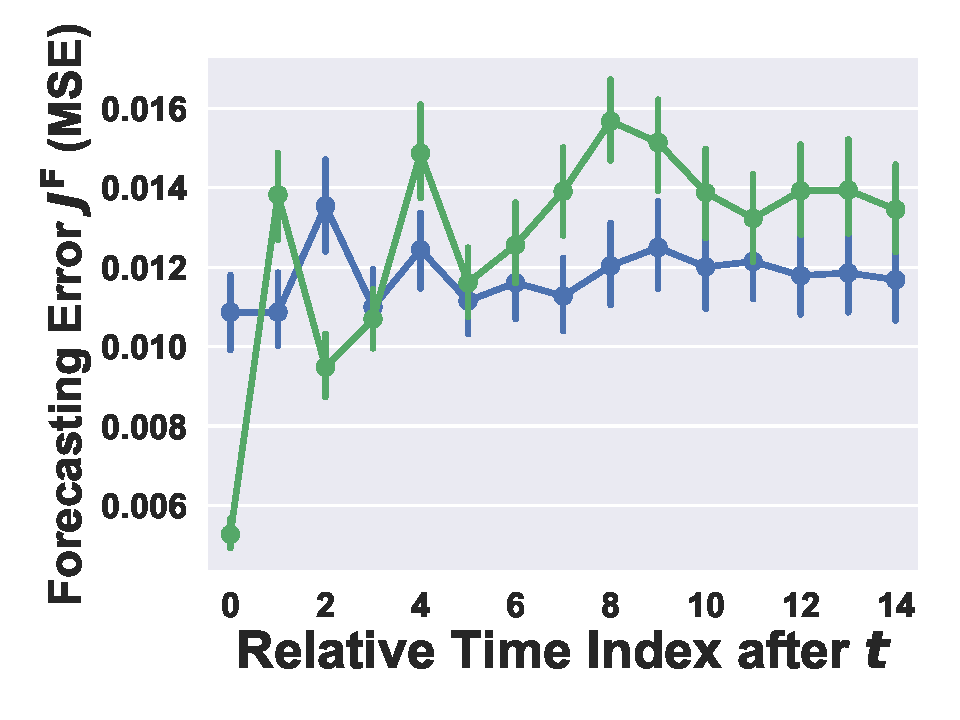
\includegraphics[width=0.31\columnwidth]{figures/cell/forecast_errors_time_horizon.pdf}}
\label{fig_cell_forecast_errors_time_horizon}
}
%\subfigure[]{
\subfigure{
{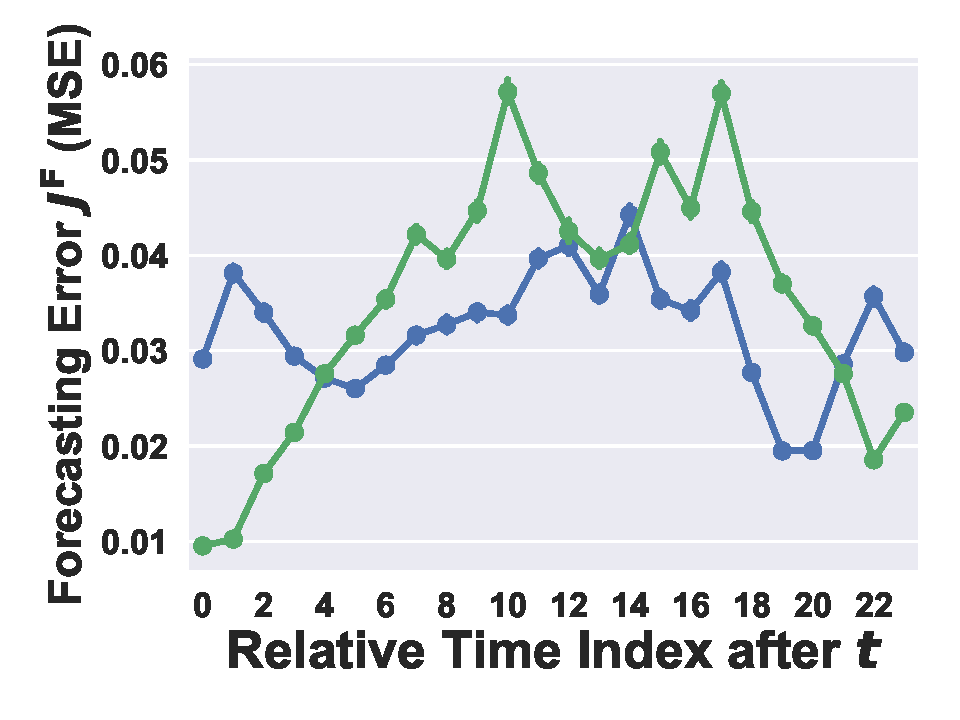
\includegraphics[width=0.31\columnwidth]{figures/pjm/forecast_errors_time_horizon.pdf}}
\label{fig_pjm_forecast_errors_time_horizon}
}
\caption{\textbf{Real-world dataset results: } From left to right, the columns correspond to smart factory regulation from IoT sensors, taxi dispatching with cell demand, and battery storage optimization. \textbf{(Row 1)} Co-design achieves lower cost $\Jcontrol$ for smaller bottlenecks $\zbottleneck$ compared to task-agnostic methods. \textbf{(Row 2)} We also achieve lower error for each dimension $i$ of the vector control, $u(i)$, plotted for a highly-compressed $Z=3$. \textbf{(Row 3)} Co-design heavily reduces forecasting errors for initial horizons that are especially important for MPC's decision-making.}
%While a task-agnostic approach (blue) distributes forecasting errors roughly evenly across a horizon $H$, our co-design approaches heavily reduce errors for initial horizons that are especially important for MPC's decision-making.}
\label{fig_real}
\end{center}
\vskip -0.2in
\end{figure*}
%Aggregated forecasting error for  each relative time index when $Z=3$, under different policies. (j-l) Forecasting error for each $s(i)$ and each relative time index when $Z=3$, under task-agnostic (top) and weighted (bottom) policy, respectively.
%\caption{Results for real data. Columns from left to right corresponds to smart home regulation, taxi dispatching and battery storage optimization, respectively. (a-c) Control cost $J$ under different bottleneck dimension $Z$ and training policies; (d-f) Control error for each $u(i)$ when $Z=3$ under different training policies; (g-i) Aggregated forecasting error for  each relative time index when $Z=3$, under different policies. (j-l) Forecasting error for each $s(i)$ and each relative time index when $Z=3$, under task-agnostic (top) and weighted (bottom) policy, respectively.}
